\hypertarget{BoundaryFF_8cpp}{\section{M3\+S\+Y\+M/\+Mechanics/\+Force\+Field/\+Boundary\+F\+F.cpp File Reference}
\label{BoundaryFF_8cpp}\index{M3\+S\+Y\+M/\+Mechanics/\+Force\+Field/\+Boundary\+F\+F.\+cpp@{M3\+S\+Y\+M/\+Mechanics/\+Force\+Field/\+Boundary\+F\+F.\+cpp}}
}
{\ttfamily \#include \char`\"{}Boundary\+F\+F.\+h\char`\"{}}\\*
{\ttfamily \#include \char`\"{}Boundary\+Repulsion.\+h\char`\"{}}\\*
{\ttfamily \#include \char`\"{}Boundary\+Repulsion\+L\+J.\+h\char`\"{}}\\*
{\ttfamily \#include \char`\"{}Boundary\+Repulsion\+Exp.\+h\char`\"{}}\\*
{\ttfamily \#include \char`\"{}Boundary\+Element.\+h\char`\"{}}\\*
{\ttfamily \#include \char`\"{}Bead.\+h\char`\"{}}\\*
Include dependency graph for Boundary\+F\+F.\+cpp\+:\nopagebreak
\begin{figure}[H]
\begin{center}
\leavevmode
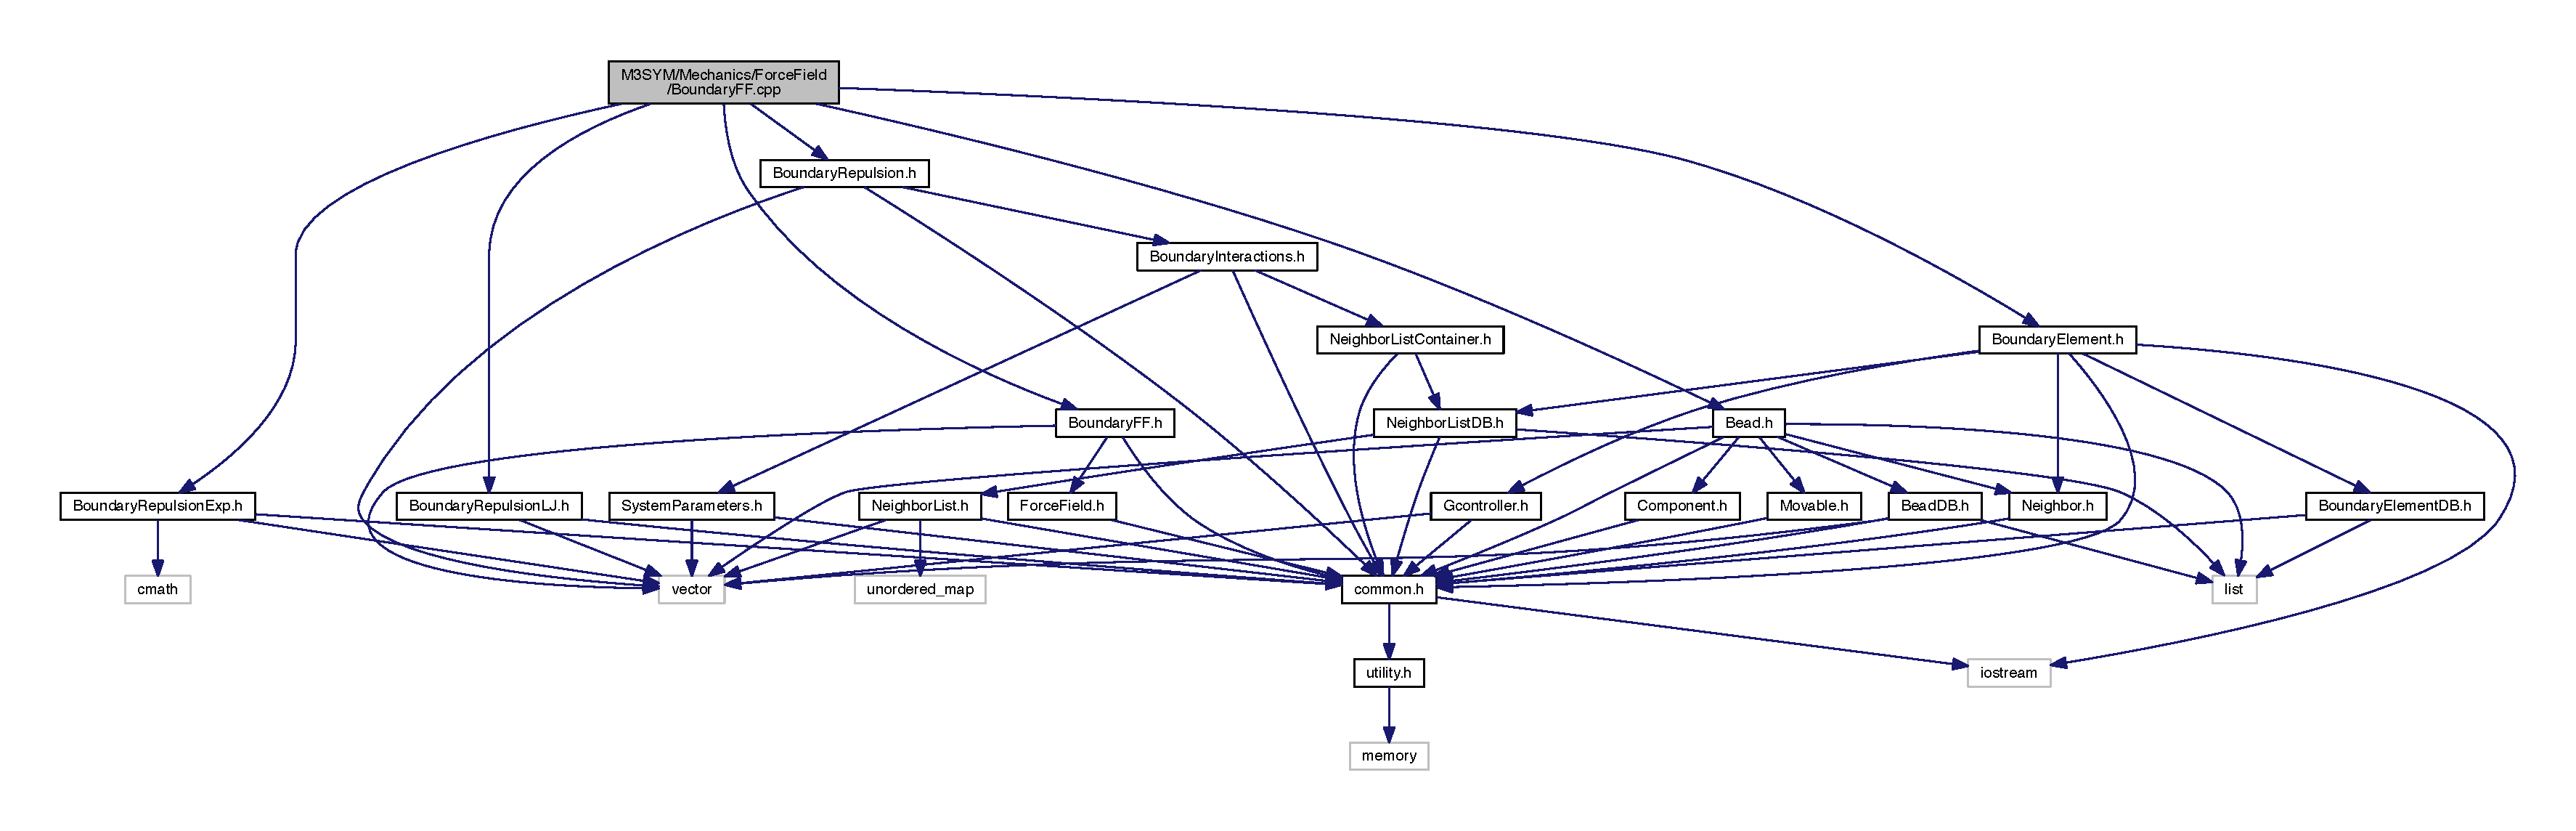
\includegraphics[width=350pt]{BoundaryFF_8cpp__incl}
\end{center}
\end{figure}
